\documentclass[12pt]{article}
\usepackage{graphicx}
\usepackage{geometry}
\usepackage{listings}
\usepackage{xcolor}
\usepackage{float}
\usepackage{amsmath}
\usepackage{tikz}
\usetikzlibrary{shapes.geometric, arrows, positioning}

\geometry{a4paper, margin=1in}

\definecolor{codegreen}{rgb}{0,0.6,0}
\definecolor{codegray}{rgb}{0.5,0.5,0.5}
\definecolor{codepurple}{rgb}{0.58,0,0.82}
\definecolor{backcolour}{rgb}{0.96,0.96,0.94}

\lstdefinestyle{mystyle}{
    backgroundcolor=\color{backcolour},   
    commentstyle=\color{codegreen},
    keywordstyle=\color{magenta},
    numberstyle=\tiny\color{codegray},
    stringstyle=\color{codepurple},
    basicstyle=\ttfamily\footnotesize,
    breakatwhitespace=false,         
    breaklines=true,                 
    captionpos=b,                    
    keepspaces=true,                 
    numbers=left,                    
    numbersep=5pt,                  
    showspaces=false,                
    showstringspaces=false,
    showtabs=false,                  
    tabsize=2
}
\lstset{style=mystyle}

\title{\textbf{Lab 6: Memory BIST (MBIST) Insertion, Synthesis, and Two-Stage LEC Verification}}
\author{R Sarang (EC23I2015)}
\date{\today}

\begin{document}

\maketitle
\tableofcontents
\newpage

\section{Overview: Memory BIST Design \& Verification Flow}

Modern System-on-Chips (SoCs) integrate large embedded SRAM arrays. Because memories have dense physical footprints with unique failure modes, testing them requires inserting dedicated built-in test hardware, known as \textbf{Memory Built-In Self-Test (MBIST)}.

In this lab, the design under test is \texttt{counter\_system}, which incorporates two synchronous single-port SRAM instances:
\begin{itemize}
    \item \texttt{u1}: \texttt{SYNC\_1RW\_256x16} (256 words $\times$ 16 bits)
    \item \texttt{u2}: \texttt{SYNC\_1RW\_64Kx8} (65536 words $\times$ 8 bits)
\end{itemize}

The complete flow consists of three major transformation phases and two formal verification stages:

\begin{figure}[H]
\centering
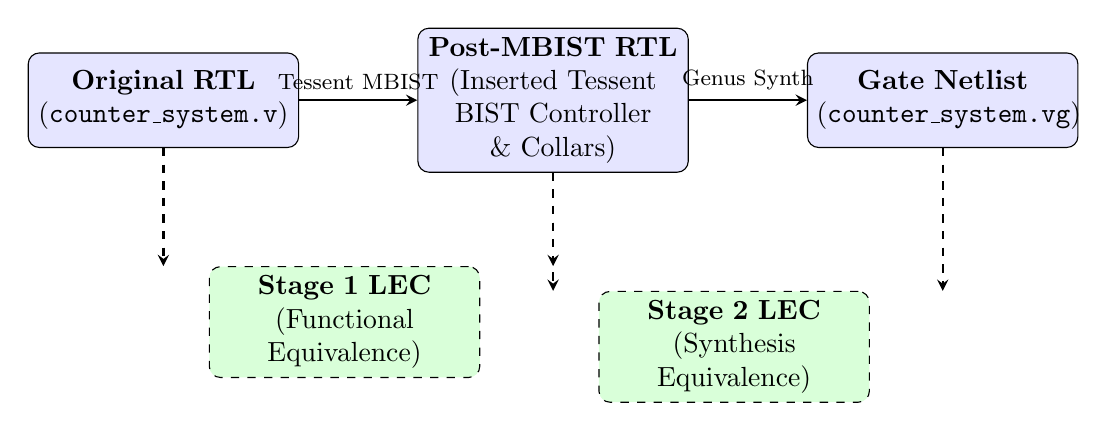
\begin{tikzpicture}[
    node distance=1.5cm,
    block/.style={rectangle, draw, fill=blue!10, text width=3.2cm, text centered, rounded corners, minimum height=1.2cm},
    arrow/.style={thick,->,>=stealth},
    verif/.style={rectangle, draw, dashed, fill=green!15, text width=3.2cm, text centered, rounded corners, minimum height=1.0cm}
]

\node (orig) [block] {\textbf{Original RTL}\\(\texttt{counter\_system.v})};
\node (mbist) [block, right=of orig] {\textbf{Post-MBIST RTL}\\(Inserted Tessent BIST Controller \& Collars)};
\node (netlist) [block, right=of mbist] {\textbf{Gate Netlist}\\(\texttt{counter\_system.vg})};

\node (lec1) [verif, below=of orig, xshift=2.3cm] {\textbf{Stage 1 LEC}\\(Functional Equivalence)};
\node (lec2) [verif, below=of mbist, xshift=2.3cm] {\textbf{Stage 2 LEC}\\(Synthesis Equivalence)};

\draw [arrow] (orig) -- node[above] {\footnotesize Tessent MBIST} (mbist);
\draw [arrow] (mbist) -- node[above] {\footnotesize Genus Synth} (netlist);

\draw [arrow, dashed] (orig.south) -- ++(0,-0.5) -| (lec1.north -| orig.south);
\draw [arrow, dashed] (mbist.south) -- ++(0,-0.5) -| (lec1.north -| mbist.south);

\draw [arrow, dashed] (mbist.south) -- ++(0,-0.5) -| (lec2.north -| mbist.south);
\draw [arrow, dashed] (netlist.south) -- ++(0,-0.5) -| (lec2.north -| netlist.south);

\end{tikzpicture}
\caption{Overall Memory BIST Implementation and Two-Stage LEC Flow}
\end{figure}

---

\section{Why is a Two-Stage LEC Verification Necessary?}

In standard ASIC design without BIST, equivalence checking is a single comparison between the golden RTL and the synthesized gate netlist:
$$\text{Golden (RTL)} \Longleftrightarrow \text{Revised (Gate Netlist)}$$

However, when MBIST is inserted at the RTL level, comparing the original pre-MBIST RTL directly against the final synthesized netlist is \textbf{practically impossible or invalid} because:
\begin{enumerate}
    \item \textbf{Significant Structural Discrepancy:} MBIST insertion adds new state machines (BIST controller \texttt{c1}), test collar multiplexers around every memory pin, and an IEEE 1149.1 / IEEE 1500 / IJTAG IEEE 1687 network (SIBs). The original RTL has none of these registers or primary I/O pins.
    \item \textbf{Failure Localization:} If a one-step comparison fails, it is impossible to determine whether the bug was caused by incorrect MBIST collar multiplexing by Tessent or improper gate optimization/retiming by Cadence Genus.
\end{enumerate}

To solve this, the equivalence check is cleanly partitioned into two distinct verification stages.

---

\section{Stage 1: Pre-MBIST RTL vs. Post-MBIST RTL}

\subsection{Objective}
To mathematically prove that the insertion of MBIST hardware (test controllers, multiplexers, and test ports) does \textbf{not alter the functional behavior} of the original counter system when the design operates in normal mission mode.

\subsection{Mechanism \& Pin Constraints}
In the post-MBIST RTL, multiplexers (called \textit{collars}) are inserted directly on the inputs of the memory macros:
\begin{itemize}
    \item When \texttt{BIST\_INPUT\_SELECT = 1}, test pattern data from the BIST controller feeds the memory.
    \item When \texttt{BIST\_INPUT\_SELECT = 0}, normal mission-mode data from the counter logic feeds the memory.
\end{itemize}

To prove functional equivalence, Cadence Conformal LEC is instructed to constrain the test logic to its inactive state in the revised design:

\begin{lstlisting}[language=Tcl, caption=Stage 1 LEC Constraints (mbist.do)]
// Constrain scan and IJTAG reset
add pin constraints 0 scan_enable -both
add pin constraints 0 scan_mode -both
add pin constraints 0 ijtag_reset -revised

// Ignore test scan-out pins
add ignored outputs ijtag_so -revised

// Force Memory BIST collars to Normal Functional Mode
add primary input u1_interface_inst/BIST_INPUT_SELECT_reg/Q -pin -revised
add primary input u2_interface_inst/BIST_INPUT_SELECT_reg/Q -pin -revised
add pin constraints 0 u1_interface_inst/BIST_INPUT_SELECT_reg/Q -revised
add pin constraints 0 u2_interface_inst/BIST_INPUT_SELECT_reg/Q -revised
\end{lstlisting}

\subsection{Results}
With the BIST multiplexers held at 0:
\begin{itemize}
    \item Primary inputs, outputs, registers, and black-box memory interfaces map 1:1.
    \item \textbf{Outcome:} \textbf{105 out of 105 compared points EQUIVALENT} (0 Non-equivalent, 0 Abort).
    \item \textbf{Conclusion:} MBIST insertion is 100\% transparent during normal mission mode.
\end{itemize}

---

\section{Stage 2: Post-MBIST RTL vs. Synthesized Gate Netlist}

\subsection{Objective}
To prove that the logic synthesis tool (Cadence Genus) accurately translated \textbf{both} the functional counter logic and the newly inserted MBIST controllers into standard cell gates (\texttt{adk.lib}) without introducing logic errors, unintended optimizations, or broken scan paths.

\subsection{Differences from Stage 1}
\begin{table}[H]
\centering
\begin{tabular}{|l|p{6.5cm}|p{6.5cm}|}
\hline
\textbf{Property} & \textbf{Stage 1 LEC} & \textbf{Stage 2 LEC} \\
\hline
\textbf{Golden Design} & Original Functional RTL (\texttt{rtl\_file\_list}) & Post-MBIST RTL (\texttt{mbist\_file\_list}) \\
\hline
\textbf{Revised Design} & Post-MBIST RTL (\texttt{mbist\_file\_list}) & Synthesized Gate Netlist (\texttt{counter\_system.vg}) \\
\hline
\textbf{Focus} & Verify that test collars preserve functional behavior in mission mode. & Verify that synthesis correctly mapped every gate, register, and BIST controller. \\
\hline
\textbf{BIST State} & Constrained to \textbf{Inactive} (\texttt{BIST\_INPUT\_SELECT = 0}) & \textbf{Unconstrained} (Both functional and test modes must match). \\
\hline
\textbf{Tool Used} & Cadence Conformal LEC & Cadence Conformal LEC \\
\hline
\end{tabular}
\caption{Comparison of Stage 1 and Stage 2 LEC Verification}
\end{table}

---

\section{Summary of Results Across the Flow}

\begin{table}[H]
\centering
\begin{tabular}{|l|l|l|}
\hline
\textbf{Phase} & \textbf{Tool} & \textbf{Status / Result} \\
\hline
MBIST Insertion & Siemens Tessent & 2 Memories wrapped; Controller \texttt{c1} created. \\
Signoff Simulation & Siemens QuestaSim & 3/3 Tests Passed (\texttt{pass 3 fail 0}). \\
Stage 1 LEC & Cadence Conformal & 105/105 Points Equivalent (0 Non-EQ). \\
Logic Synthesis & Cadence Genus & Completed cleanly; Reports generated. \\
Stage 2 LEC & Cadence Conformal & Post-MBIST RTL $\equiv$ Gate Netlist (\texttt{.vg}). \\
\hline
\end{tabular}
\caption{Verification Status Summary}
\end{table}

\end{document}
